With a goal of recreating findings of O'Neil et al. \cite{lruk} we evaluated LRU-1, LRU-2 and LRU-3 algorithms on three workloads:
\begin{itemize}
\item a synthetic workload simulating alternating references to two pools' pages with different frequencies,
\item a synthetic workload simulating random accesses according to Zipfian 80-20 distribution, and
\item buffer accesses captured with instrumented PostgreSQL running \texttt{pgbench}.
\end{itemize}

To support our hypotheses that LRU-2 and LRU-3 outperform LRU-1 on database workloads, we expect our results to show higher hit ratio for all buffer sizes in LRU-2 and LRU-3 case. We also expect to see the difference in performance decrease as buffer size grows, since in the limit of infinite buffer size, they should all perform the same.

Our second hypothesis is that LRU-2 and LRU-3 performances are similar. We don't expect to see high differences in cache hit ratio in any workload.

We present results for these workloads in the following sections.

\subsection{Two Pool Experiment}

As our first experiment, we replicated the two-pool experiment conducted by O'Neil et al. \cite{lruk}. They considered two pools of pages, Pool 1 with size $N_1$ and Pool 2 with $N_2$ pages and simulated random alternating accesses to those pools. With $N_1 << N_2$, the goal of this experiment was to simulate alternating accesses to index and record pages. Specifically, on every even access they uniformly choose one page from Pool 1 and on every odd access they choose one page from Pool 2. Thus, every page from Pool 1 has probability of reference $\frac{1}{2N_1}$ and every page from Pool 2 $\frac{1}{2N_2}$.

We replicated the experiment exactly, using $N_1 = 100$ and $N_2 = 10000$ pages. Figure \ref{fig:two_pool} shows measured hit rates for specific buffer sizes. Our results are consistent with O'Neil et al. \cite{lruk}, where they found that LRU-1 has lower hit rates than LRU-2 and LRU-3 for a given buffer size. We also see that LRU-1 performance approaches LRU-2 and LRU-3 on larger buffer sizes. LRU-2 and LRU-3 performances are similar, with LRU-3 slightly outperforming LRU-2. However, O'Neil et al. argue that the difference is too small to be traded for the slower responsiveness which LRU-3 exhibits on evolving and dynamic access patterns.

\begin{figure}[t!]
    \centering
	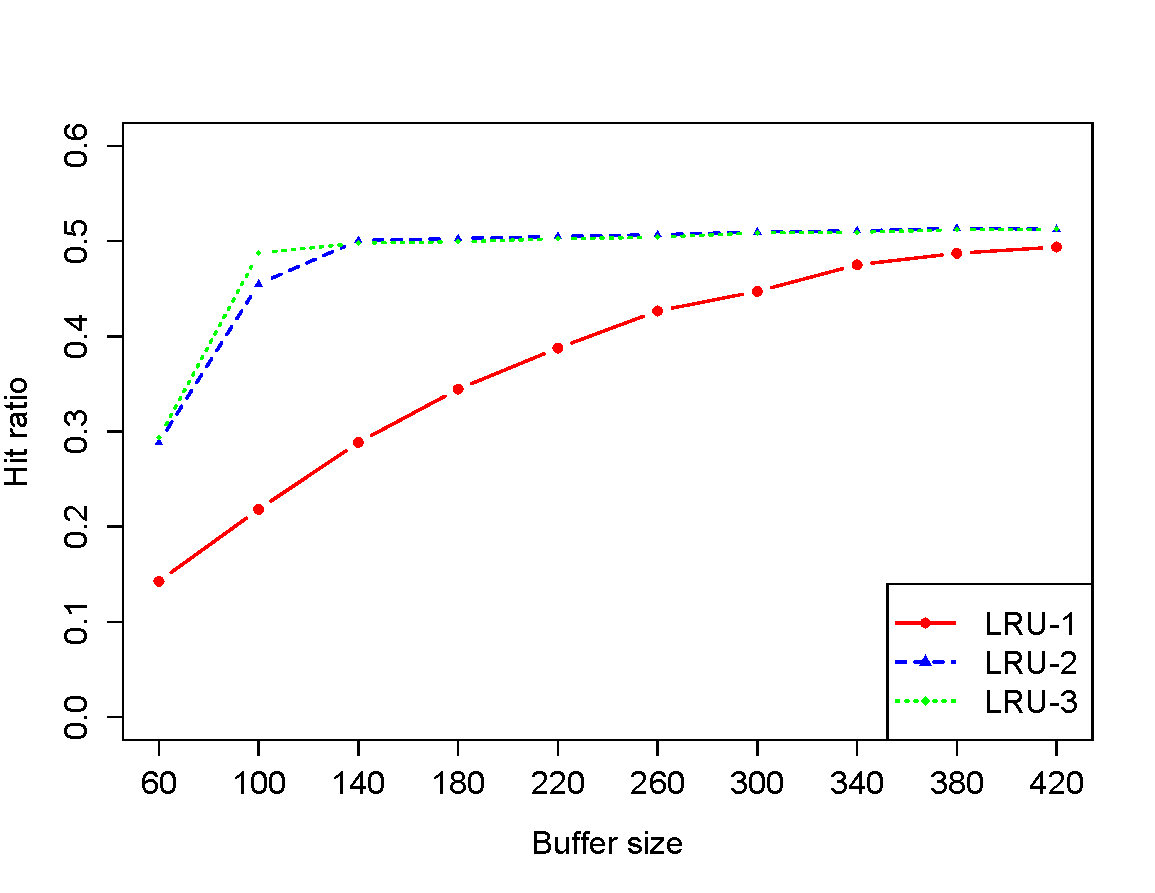
\includegraphics[width=0.5\textwidth]{./figures/two_pool.pdf}
	\caption{Simulation results of two-pool experiment with disk page pools of $N_1 = 100$ pages and $N_2 = 10000$ pages. The horizontal axis shows the simulate buffer size and the vertical axis shows measured hit ratio. All measurements were evaluated with Correlated Reference Period set to 0.}
	\label{fig:two_pool}
\end{figure}


\subsection{Zipfian Random Access Experiment}

Next, we evaluated LRU-K on workloads that access pages according to Zipfian distribution, replicating the experiment conducted by O'Neil et al. \cite{lruk}. They used $N = 1000$ pages numbered 1 through N; the probability for referencing a page with page number less than or equal to i was $\left(\frac{i}{N}\right)^\frac{\log{a}}{\log{b}}$ with constants $a = 0.8$ and $b = 0.2$.

Their findings were that LRU-2 gains are lower than in the two-pool test, since the skew of Zipfian 80-20 distribution is milder than skew in the two-pool test. Figure \ref{fig:zipfian} shows the hit ratios we measured for different buffer sizes. There are three main points we can take from this figure. First, LRU-2 and LRU-3 clearly outperform LRU-1, more so for smaller buffer sizes. Second, LRU-2 and LRU-3 performances are similar. Third, gains for LRU-2 are smaller than in two pool experiment.

Our first and third findings are consistent with O'Neil et al. They didn't evaluate LRU-3 against a Zipfian distribution, so we cannot compare our second finding.

\begin{figure}[t!]
    \centering
	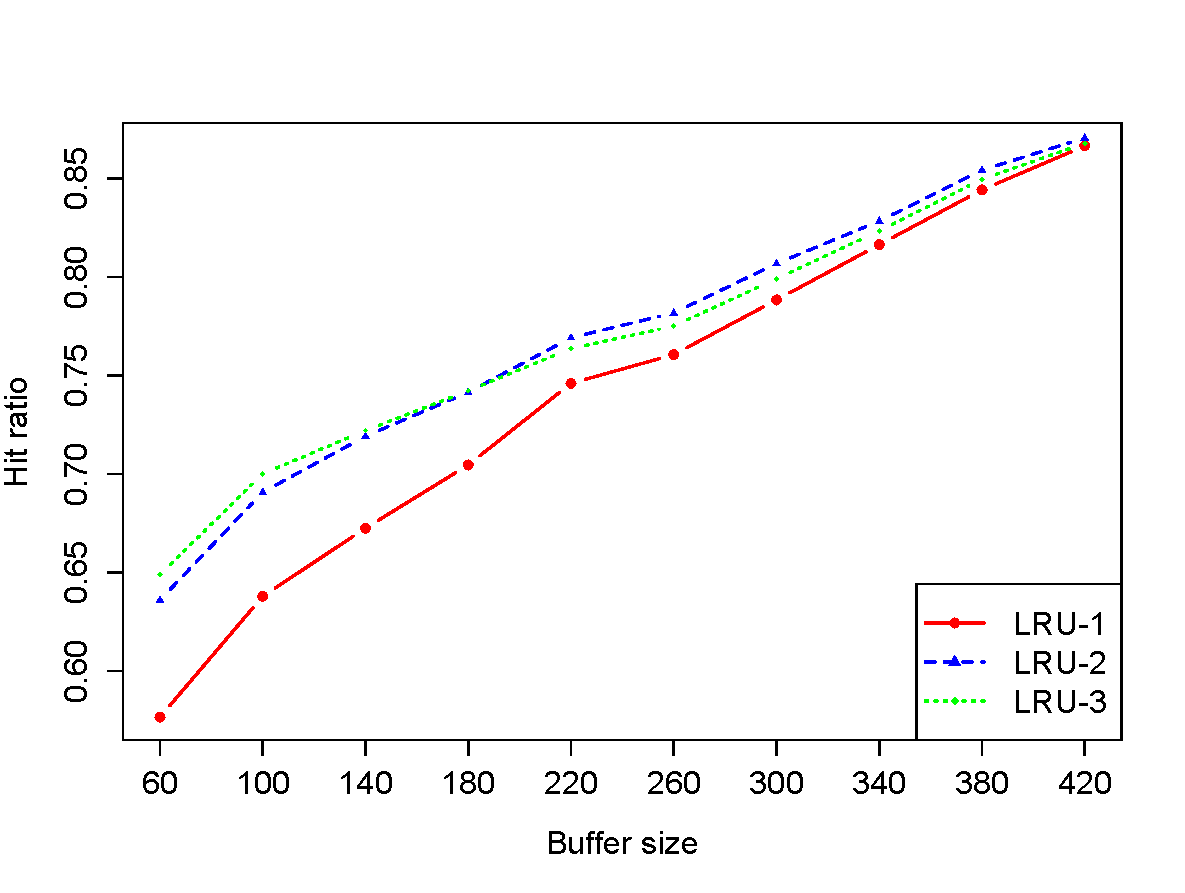
\includegraphics[width=0.5\textwidth]{./figures/zipfian.pdf}
	\caption{Simulation results of cache hit ratio for random access with Zipfian 80-20 distribution to $N = 1000$ pages in the pool. The horizontal axis shows the simulated buffer size and the vertical axis shows measured hit ratio. All measurements were evaluated with Correlated Reference Period set to 0.}
	\label{fig:zipfian}
\end{figure}


\subsection{PostgreSQL Trace Experiment}

For their third experiment, O'Neil et al. \cite{lruk} used a trace from the OLTP system of a large bank. We did not have access to this trace, so we could not replicate the experiment exactly. Instead, we instrumented PostgreSQL to capture all buffer accesses and ran \texttt{pgbench} benchmark with 400 clients, each issuing 10 transactions. This workload generated a total of 89692 accesses. However, because PostgreSQL's \texttt{elog} function isn't thread-safe, some parts of our trace were corrupted. As a result, we captured only 87373 accesses, which is 97.4\% of total buffer accesses. We tried to make \texttt{elog} thread-safe, but that resulted in big slowdowns of the system, causing some transactions to be aborted.

We evaluated the LRU-1, LRU-2 and LRU-3 algorithms on the generated trace. For LRU-2 and LRU-3, we ran two experiments, one with Correlated Reference Period (CRP) set to be 0 and another with $CRP = 20$. With $CRP = 20$, we collapse any two consecutive references into one page reference when there are no more than 19 other page references between them. Details of the Correlated Reference Period are discussed in \cite{lruk}. Since we had only one trace, we ran the experiment only once and report the hit ratio of that run (unlike in previous experiments, where we reported average of four runs). Figure \ref{fig:postgres} shows the hit rates we measured for different buffer sizes. It is interesting to note is that LRU-2 and LRU-3 are inferior to LRU-1 with $CRP = 0$. However, with $CRP = 20$ they both outperform LRU-1. Unfortunately, O'Neil et al. \cite{lruk} never stated which CRP they used in their experiments nor suggested how to set suitable CRP under different workloads.

\begin{figure}[t!]
    \centering
	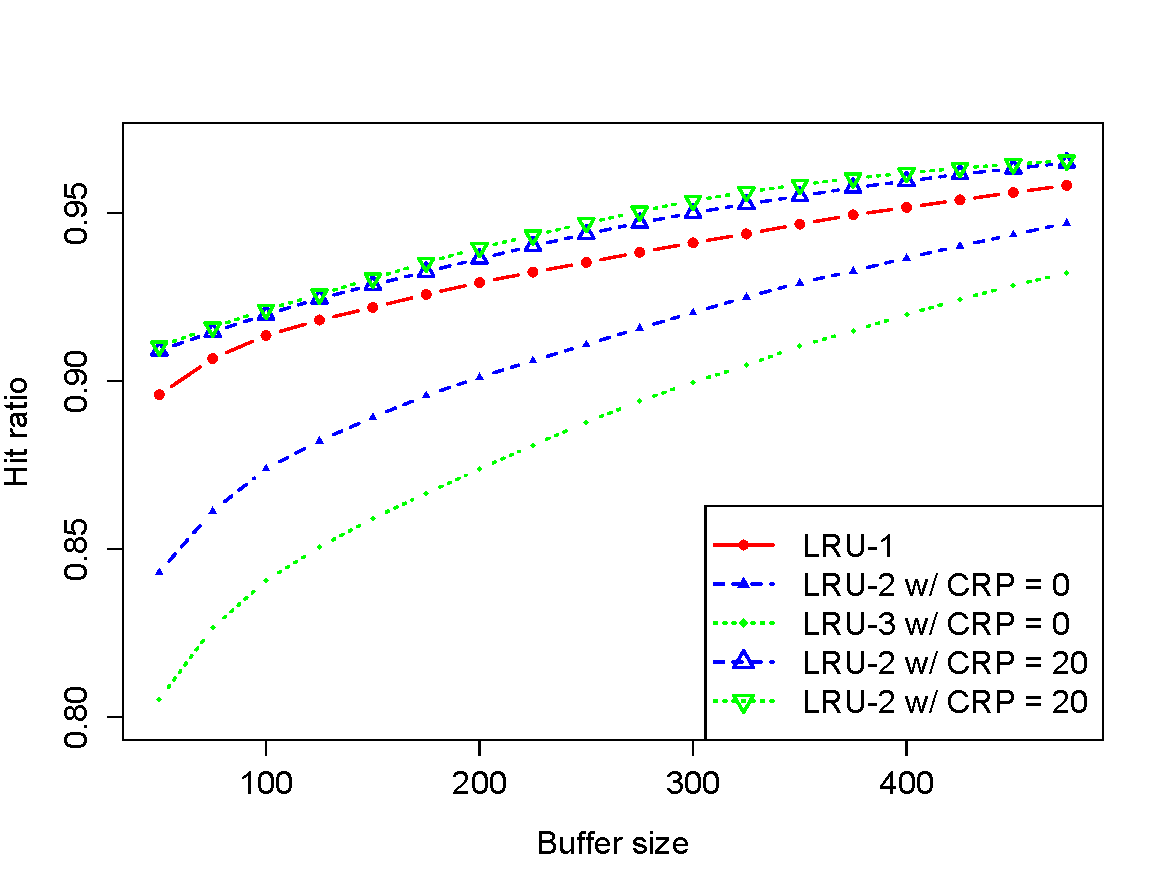
\includegraphics[width=0.5\textwidth]{./figures/postgres.pdf}
	\caption{Simulation results of different buffer management strategies using a trace collected from PostgreSQL running \texttt{pgbench} benchmark. The horizontal axis shows the simulated buffer size and the vertical axis shows measured hit ratio. LRU-2 and LRU-3 were evaluated with Correlated Reference Period set to 0 and 20.}
	\label{fig:postgres}
\end{figure}
